\lstset{ %
  backgroundcolor=\color{white},   % choose the background color; you must add \usepackage{color} or \usepackage{xcolor}
  basicstyle=\footnotesize,             % the size of the fonts that are used for the code
  breakatwhitespace=false,            % sets if automatic breaks should only happen at whitespace
  breaklines=true,                 	   % sets automatic line breaking
  captionpos=b,                    	   % sets the caption-position to bottom
  commentstyle=\color{dkgreen},   % comment style
  deletekeywords={...},            	   % if you want to delete keywords from the given language
  escapeinside={\%*}{*)},             % if you want to add LaTeX within your code
  extendedchars=true,                    % lets you use non-ASCII characters; for 8-bits encodings only, does not work with UTF-8
  frame=single,	                        % adds a frame around the code
  keepspaces=true,                         % keeps spaces in text, useful for keeping indentation of code (possibly needs columns=flexible)
  keywordstyle=\color{blue},          % keyword style
  otherkeywords={*,...},                % if you want to add more keywords to the set
  numbers=left,                               % where to put the line-numbers; possible values are (none, left, right)
  numbersep=5pt,                           % how far the line-numbers are from the code
  numberstyle=\tiny\color{gray},   % the style that is used for the line-numbers
  rulecolor=\color{black},                % if not set, the frame-color may be changed on line-breaks within not-black text (e.g. comments (green here))
  showspaces=false,                       % show spaces everywhere adding particular underscores; it overrides 'showstringspaces'
  showstringspaces=false,              % underline spaces within strings only
  showtabs=false,                           % show tabs within strings adding particular underscores
  stepnumber=1,                             % the step between two line-numbers. If it's 1, each line will be numbered
  stringstyle=\color{mauve},          % string literal style
  tabsize=2,	                                  % sets default tabsize to 2 spaces
  title=\lstname                               % show the filename of files included with \lstinputlisting; also try caption instead of title
}

\chapter{DL4J-Projekt in IntelliJ aufsetzen}
{
Nach erfolgreicher Installation von IntelliJ und Maven kann ein DL4J-Projekt mithilfe von Maven eingerichtet werden. Hierf"ur w"ahlt man \glqq File\grqq{} $\rightarrow$ \glqq New\grqq{} $\rightarrow$ \glqq Project ...\grqq . 
\renewcommand{\figurename}{Abb.}
\begin{figure}[htp]
%%\begin{floatingfigure}[r]{textwidth}
\centering
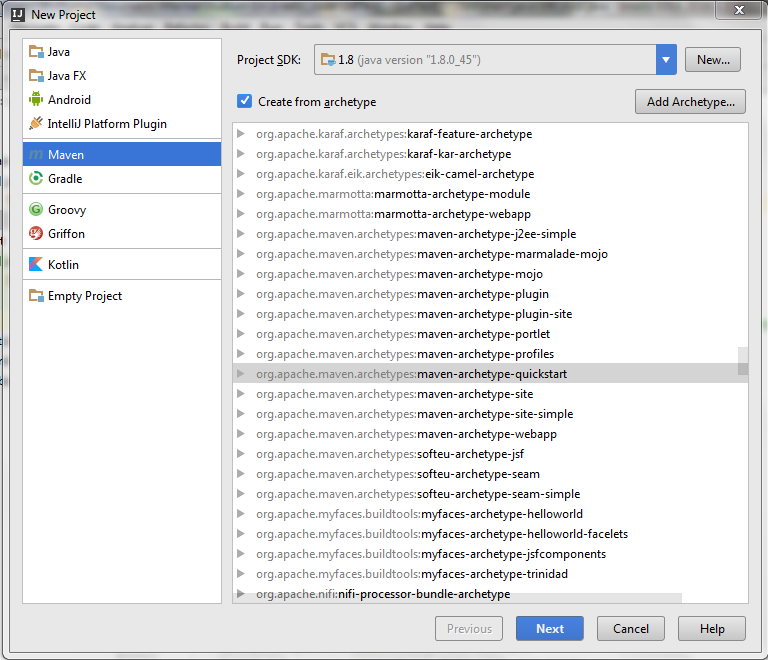
\includegraphics[width=0.80\textwidth]{pictures/mavenProj.png}
\caption[\glqq New Project\grqq{} Fenster]{\glqq New Project\grqq{} Fenster}
%%\end{floatingfigure} 
\end{figure}
Es "offnet sich das \glqq New Project\grqq -Fenster, wie in Abbildung A.1 abgebildet und man w"ahlt auf der linken Seite \glqq Maven\grqq{} (in der Abbildung mit einer roten 1 versehen). Das K"astchen \glqq Create from archetype\grqq{} (in Abbildung gekennzeichnet mit 2) wird ausgew"ahlt und aus der Liste, der verf"ugbaren Typen der Typ \glqq maven-archetype-quickstart\grqq{} (in Abbildung gekennzeichnet mit 3) gew"ahlt. Danach auf \glqq Next\grqq{}  und die GroupId (Package Name) sowie ArtifactId (?) festlegen. Anschlie{\ss}end noch einen Projektname festlegen und \glqq Finish\grqq{} dr"ucken.

http://nd4j.org/getstarted.html

Nachdem Maven f"ur einen die Projektstruktur erstellt hat, muss man die neu erstellte POM.xml Datei noch anpassen. Die POM.xml enth"alt die Projektabh"angigkeiten, welche je Projekt variieren k"onnen. Hier kann man festlegen ob das Projekt auf der CPU oder GPU laufen soll.


The default backend for CPUs is nd4j-native. You can paste that into the $<$dependencies$>$ ... $<$/dependencies$>$ section of your POM like this:
\lstset{language=XML}
\begin{lstlisting}[language=XML,caption=applicationContext.xml]
 <dependency>
   <groupId>org.nd4j</groupId>
   <artifactId>nd4j-native</artifactId>
   <version>${nd4j.version}</version>
 </dependency>
\end{lstlisting}

ND4J’s version is a variable here. It will refer to another line higher in the POM, in the $<$properties$>$ ... 
$<$/properties$>$ section, specifying the nd4j version and appearing similar to this:
\begin{lstlisting}[language=XML,caption=applicationContext.xml]
  <nd4j.version>0.4-rc3.9</nd4j.version>
  <dl4j.version>0.4-rc3.10</dl4j.version>
\end{lstlisting}

The DL4J dependencies you add to the POM will vary with the nature of your project.

In addition to the core dependency, given below, you may also want to install deeplearning4j-cli for the command-line interface, deeplearning4j-scaleout for running parallel on Hadoop or Spark, and others as needed.
\begin{lstlisting}[language=XML,caption=applicationContext.xml]
	   <dependency>
	     <groupId>org.deeplearning4j</groupId>
	     <artifactId>deeplearning4j-core</artifactId>
	     <version>${dl4j.version}</version>
	   </dependency>
\end{lstlisting}

Weitere Informationen bez"uglich GPU Betrieb oder Benutzung andere Betriebssysteme k"onnen auf der \cite{ND4J} Seite nachgeschlagen werden.
}